\documentclass[aspectratio=169,14pt]{beamer}
\usepackage{beamerthemeTalentSprint}
\usepackage{graphicx}
\usepackage{geometry}
\usepackage{graphics}
\usepackage{xcolor}
\usepackage{ragged2e}
\usepackage{csquotes}
\usetikzlibrary{snakes}
\title[Ensemble Methods]{Ensemble Methods}

\begin{document}
{ \1
\begin{frame}
	\title[Ensemble Methods]{Ensemble Methods}
\subtitle{Bagging}
\maketitle
\end{frame}
}

\begin{frame}{Bagging: Bootstrap Aggregation}
\begin{columns}
	\begin{column}{0.58\textwidth}
\begin{itemize}
\item<1-> \alert{Bootstrap:} Sampling the training data with replacement (N,\textless N)
\item<2-> Sample training data, D\textsubscript{i}, k times
	\begin{itemize}
		\item<4-> Train a classifier, C\textsubscript{i} on D\textsubscript{i}.
	\end{itemize}
\item<7-> Each test sample is classified by k classifiers
\item<8-> Results are averaged to obtain the final decision
\end{itemize}
	\end{column}
	\begin{column}{0.42\textwidth}
        \only<1,2>{\vspace{0.2cm}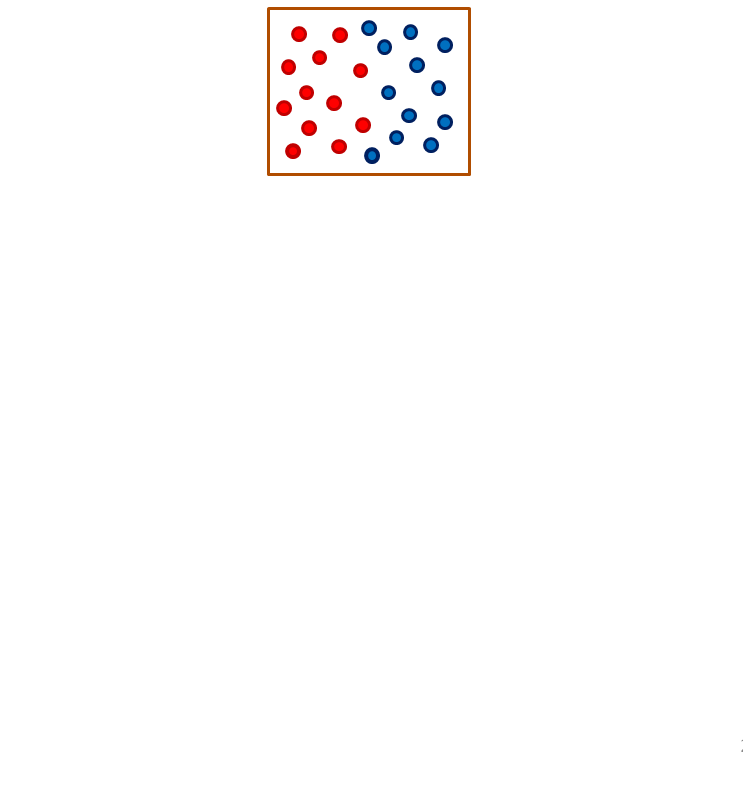
\includegraphics[width=0.9\textwidth]{Images/AIML_EM_IMG1.png}}
        \only<3,4>{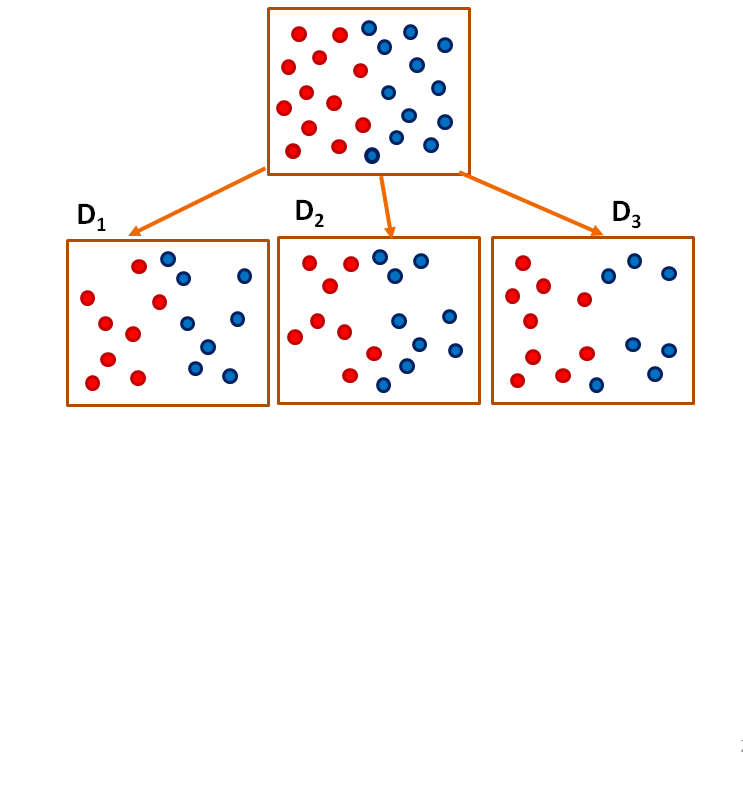
\includegraphics[width=0.9\textwidth]{Images/AIML_EM_IMG2.png}}
	\only<5>{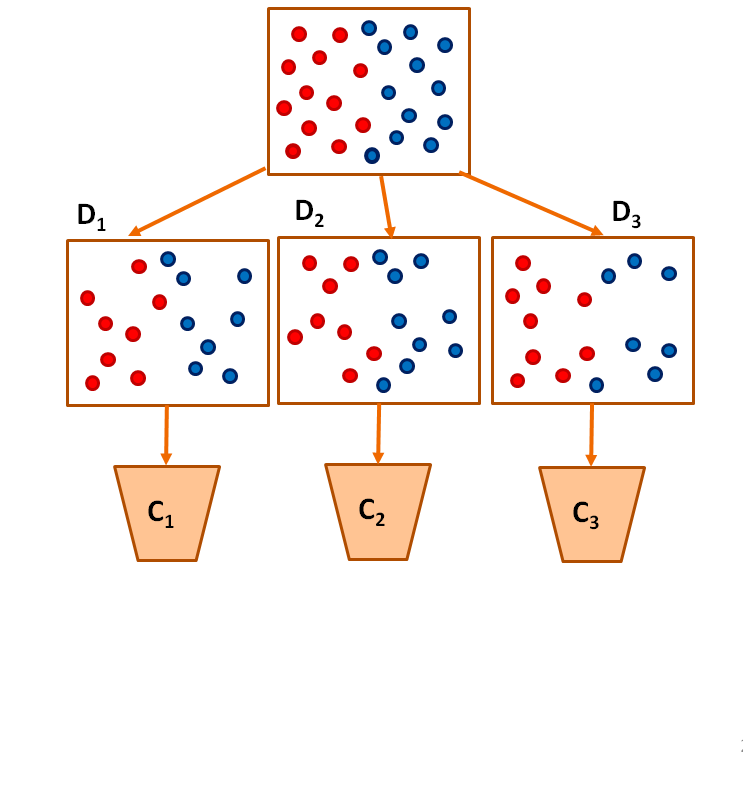
\includegraphics[width=0.9\textwidth]{Images/AIML_EM_IMG3.png}}
\only<6-8>{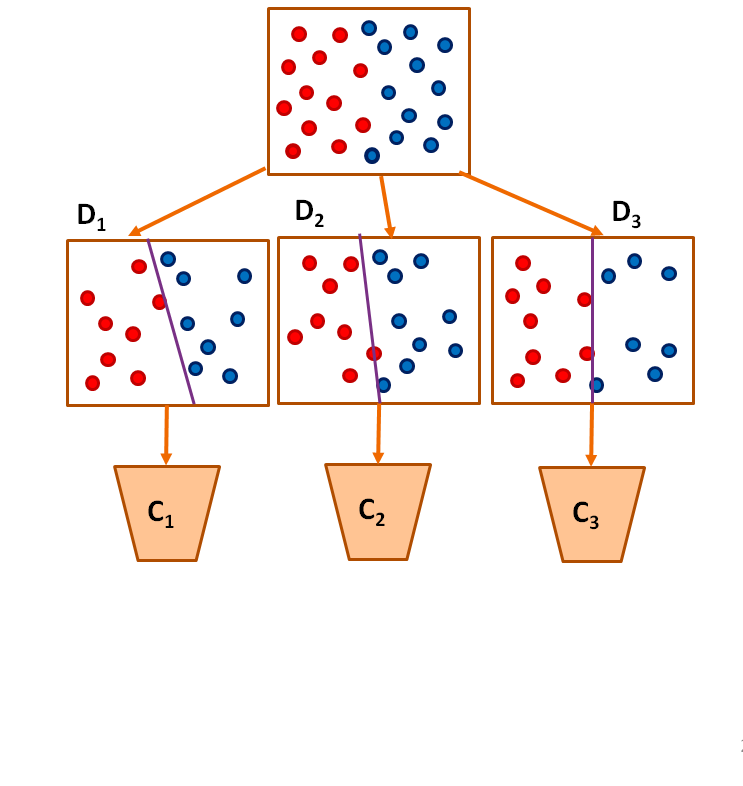
\includegraphics[width=0.9\textwidth]{Images/AIML_EM_IMG4.png}}
\only<9>{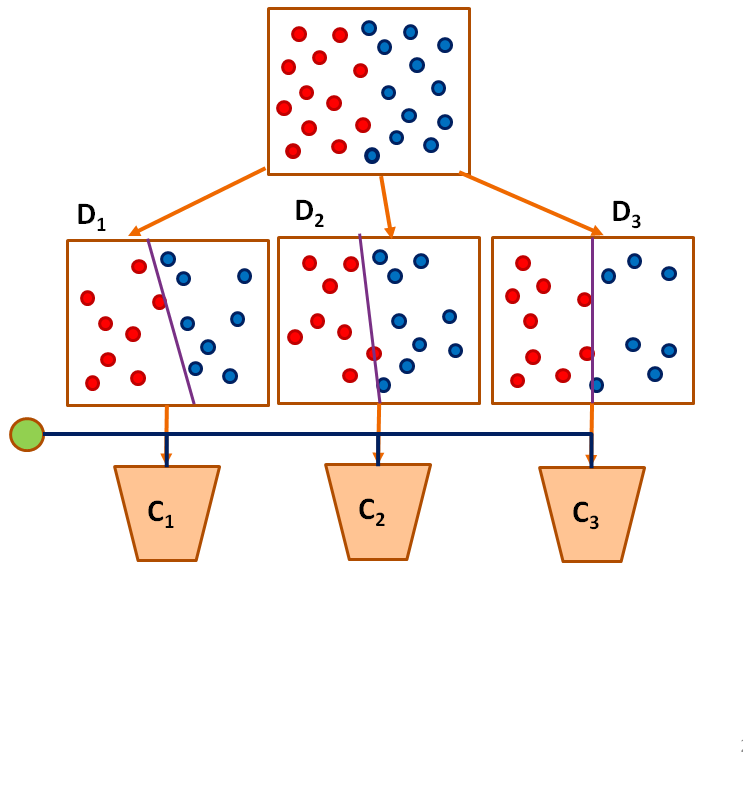
\includegraphics[width=0.9\textwidth]{Images/AIML_EM_IMG5.png}}
\only<10>{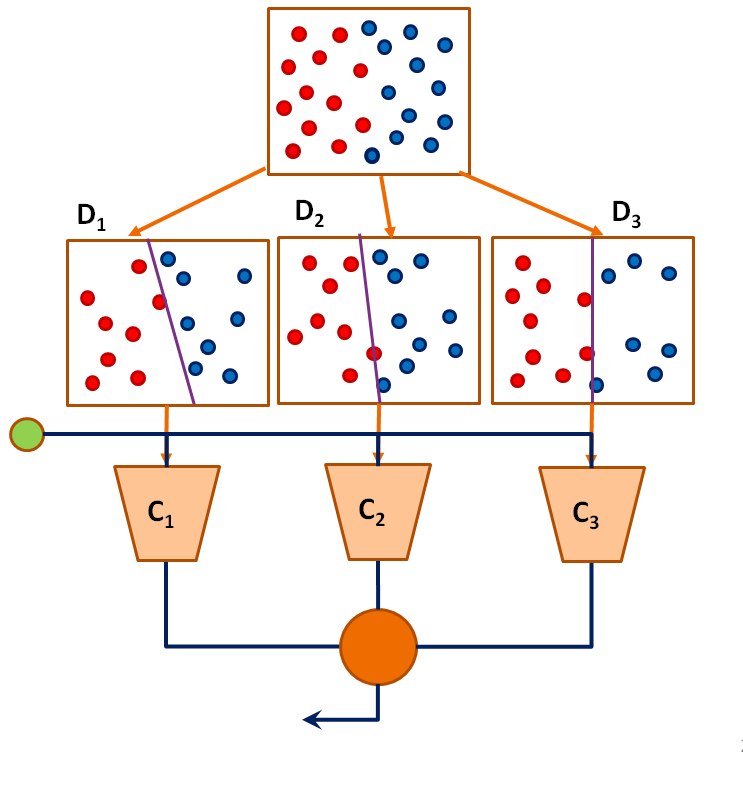
\includegraphics[width=0.9\textwidth]{Images/AIML_EM_IMG6.png}}
	\end{column}
\end{columns}
\end{frame}


\begin{frame}{Bagging}
	\begin{itemize}
		\item Bagging or \textit{bootstrap aggregation} a technique for reducing the variance of an estimated prediction function.
		\item \alert{Bootstrap:} Randomly draw datasets \alert{\textit{with replacement}} from the training data, each sample \alert{\textit{the same size as the original training set}}
		\item For classification, a \textit{committee} of trees each cast a vote for the predicted class.
	\end{itemize}
\end{frame}



{ \1
\begin{frame}
	\title[Random Forests] {Random Forests}
\subtitle{A simple way of combining Decision Trees}
\maketitle
\end{frame}
}

\begin{frame}{CART Algorithm: A Recap}
\begin{itemize}
\item Classification and Regression Trees (Leo Breiman)
\item \alert{Recursive Binary Splitting:} Greedy Algorithm
\begin{itemize}
\item All values of an attribute are sorted and all split points are tested
\item Test all such attributes and select the split with lowest cost
\end{itemize}
\item \alert{Cost Functions:}
\begin{itemize}
\item Regression:MSE
\item Classification: Gini
\end{itemize}
\end{itemize}
\end{frame}


\begin{frame}{Random Forest}
\begin{itemize}
\item \textbf{Random forest} (or \textbf{random forests}) is an ensemble classifier that consists of many decision trees and outputs the class that is the mode of the class's output by individual trees.
\item The term came from \textbf{random decision forests} that was first proposed by Tin Kam Ho of Bell Labs in 1995.
\item The method combines Breiman's "bagging" idea and the random selection of features.
\end{itemize}
\end{frame}


\begin{frame}{Random Forest}
\begin{columns}
\column{11cm}
\begin{overlayarea}{\paperwidth}{7cm}
\includegraphics<1>[width=10cm]{Images/AIML_RF_IMG7.png}
\includegraphics<2>[width=10cm]{Images/AIML_RF_IMG8.png}
\includegraphics<3>[width=10cm]{Images/AIML_RF_IMG9.png}
\end{overlayarea}
\end{columns}
\end{frame}


\begin{frame}{Random Forest}
\begin{columns}
\column{0.45\paperwidth}
Random forest classifier, an extension to bagging which uses \textit{de-correlated} trees.
\column{0.45\paperwidth}
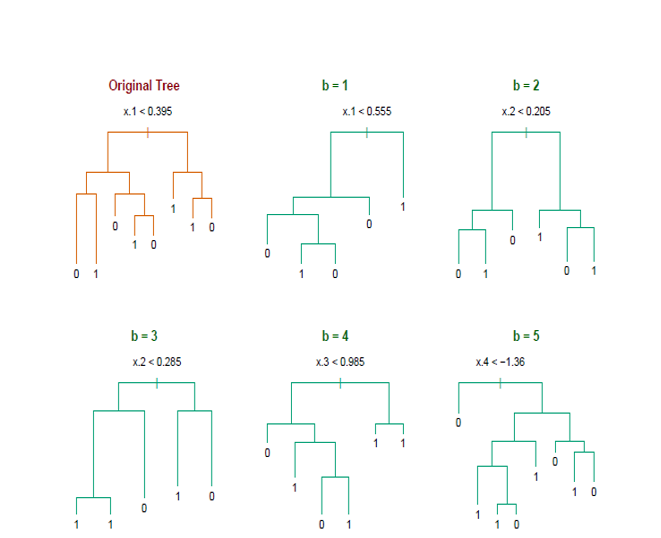
\includegraphics[width=6cm]{Images/AIML_RF_IMG10.png}
\end{columns}
\end{frame}


\begin{frame}{Random Forest Classifier}

\begin{columns}
\column{11cm}
\begin{overlayarea}{\paperwidth}{7cm}
\includegraphics<1>[width=9cm]{Images/AIML_RF_IMG11.png}
\includegraphics<2>[width=9cm]{Images/AIML_RF_IMG12.png}
\includegraphics<3>[width=9cm]{Images/AIML_RF_IMG13.png}
\includegraphics<4>[width=9cm]{Images/AIML_RF_IMG14.png}
\includegraphics<5>[width=9cm]{Images/AIML_RF_IMG15.png}
\end{overlayarea}
\end{columns}
\end{frame}



\begin{frame}{Example: Email Classification}
\begin{block}{Spam vs Ham}
\begin{itemize}
\item \alert{Features:}  2-million dimensional  (one-hot)
\item<2-> Each tree selects a subset of features (words)
\begin{itemize}
\item<3-> Select the best from the subset
\end{itemize}
\item<4-> Should the words be uniformly sampled?
\item<5-> Automatically selects relevant words
\item<6-> What is the equivalent in classification with Gene data
\end{itemize}
\end{block}
\end{frame}

{\1
\begin{frame}[plain,noframenumbering]
\title{Thanks!}
\subtitle{Questions?}
  \titlepage
\end{frame}
}

\end{document}


%\begin{frame}
%       \tikz{\draw[snake=triangles] (0,0) -- (3,0);}
%\end{frame}

